%% LyX 2.3.6.2 created this file.  For more info, see http://www.lyx.org/.
%% Do not edit unless you really know what you are doing.
\documentclass[english,aspectratio=169]{beamer}
\usepackage{mathptmx}
\usepackage{eulervm}
\usepackage[T1]{fontenc}
\usepackage[latin9]{inputenc}
\usepackage{babel}
\usepackage{amstext}
\usepackage{amssymb}
\usepackage{graphicx}
\ifx\hypersetup\undefined
  \AtBeginDocument{%
    \hypersetup{unicode=true,pdfusetitle,
 bookmarks=true,bookmarksnumbered=false,bookmarksopen=false,
 breaklinks=false,pdfborder={0 0 0},pdfborderstyle={},backref=false,colorlinks=true,
 allcolors=NYUPurple,urlcolor=LightPurple}
  }
\else
  \hypersetup{unicode=true,pdfusetitle,
 bookmarks=true,bookmarksnumbered=false,bookmarksopen=false,
 breaklinks=false,pdfborder={0 0 0},pdfborderstyle={},backref=false,colorlinks=true,
 allcolors=NYUPurple,urlcolor=LightPurple}
\fi

\makeatletter


%%%%%%%%%%%%%%%%%%%%%%%%%%%%%% LyX specific LaTeX commands.
%% Because html converters don't know tabularnewline
\providecommand{\tabularnewline}{\\}

%%%%%%%%%%%%%%%%%%%%%%%%%%%%%% Textclass specific LaTeX commands.
% this default might be overridden by plain title style
\newcommand\makebeamertitle{\frame{\maketitle}}%
% (ERT) argument for the TOC
\AtBeginDocument{%
  \let\origtableofcontents=\tableofcontents
  \def\tableofcontents{\@ifnextchar[{\origtableofcontents}{\gobbletableofcontents}}
  \def\gobbletableofcontents#1{\origtableofcontents}
}

%%%%%%%%%%%%%%%%%%%%%%%%%%%%%% User specified LaTeX commands.
\usetheme{CambridgeUS} 
\beamertemplatenavigationsymbolsempty


% Set Color ==============================
\definecolor{NYUPurple}{RGB}{87,6,140}
\definecolor{LightPurple}{RGB}{165,11,255}


\setbeamercolor{title}{fg=NYUPurple}
%\setbeamercolor{frametitle}{fg=NYUPurple}
\setbeamercolor{frametitle}{fg=NYUPurple}

\setbeamercolor{background canvas}{fg=NYUPurple, bg=white}
\setbeamercolor{background}{fg=black, bg=NYUPurple}

\setbeamercolor{palette primary}{fg=black, bg=gray!30!white}
\setbeamercolor{palette secondary}{fg=black, bg=gray!20!white}
\setbeamercolor{palette tertiary}{fg=gray!20!white, bg=NYUPurple}

\setbeamertemplate{headline}{}

\setbeamercolor{parttitle}{fg=NYUPurple}
\setbeamercolor{sectiontitle}{fg=NYUPurple}
\setbeamercolor{sectionname}{fg=NYUPurple}
\setbeamercolor{section page}{fg=NYUPurple}

\AtBeginSection[]{
  \begin{frame}
    \frametitle{Table of Contents}
    \tableofcontents[currentsection]
  \end{frame}

  % \begin{frame}
  % \vfill
  % \centering
  % \begin{beamercolorbox}[sep=8pt,center,shadow=true,rounded=true]{title}
  %   \usebeamerfont{title}\insertsectionhead\par%
  % \end{beamercolorbox}
  % \vfill
  % \end{frame}
}

\makeatother

\begin{document}
\global\long\def\reals{\mathbf{R}}%
 
\global\long\def\integers{\mathbf{Z}}%
 
\global\long\def\naturals{\mathbf{N}}%
 
\global\long\def\rationals{\mathbf{Q}}%
 
\global\long\def\ca{\mathcal{A}}%
 
\global\long\def\cb{\mathcal{B}}%
 
\global\long\def\cc{\mathcal{C}}%
 
\global\long\def\cd{\mathcal{D}}%
 
\global\long\def\ce{\mathcal{E}}%
 
\global\long\def\cf{\mathcal{F}}%
 
\global\long\def\cg{\mathcal{G}}%
 
\global\long\def\ch{\mathcal{H}}%
 
\global\long\def\ci{\mathcal{I}}%
 
\global\long\def\cj{\mathcal{J}}%
 
\global\long\def\ck{\mathcal{K}}%
 
\global\long\def\cl{\mathcal{L}}%
 
\global\long\def\cm{\mathcal{M}}%
 
\global\long\def\cn{\mathcal{N}}%
 
\global\long\def\co{\mathcal{O}}%
 
\global\long\def\cp{\mathcal{P}}%
 
\global\long\def\cq{\mathcal{Q}}%
 
\global\long\def\calr{\mathcal{R}}%
 
\global\long\def\cs{\mathcal{S}}%
 
\global\long\def\ct{\mathcal{T}}%
 
\global\long\def\cu{\mathcal{U}}%
 
\global\long\def\cv{\mathcal{V}}%
 
\global\long\def\cw{\mathcal{W}}%
 
\global\long\def\cx{\mathcal{X}}%
 
\global\long\def\cy{\mathcal{Y}}%
 
\global\long\def\cz{\mathcal{Z}}%
 
\global\long\def\ind#1{1(#1)}%
 %\newcommand{\pr}{P}
\global\long\def\pr{\mathbb{P}}%
 
\global\long\def\predsp{\cy}%
 %{\hat{\cy}}
\global\long\def\outsp{\cy}%

\global\long\def\prxy{P_{\cx\times\cy}}%
 
\global\long\def\prx{P_{\cx}}%
 
\global\long\def\prygivenx{P_{\cy\mid\cx}}%
 %\newcommand{\ex}{E}
\global\long\def\ex{\mathbb{E}}%
 
\global\long\def\var{\textrm{Var}}%
 
\global\long\def\cov{\textrm{Cov}}%
 
\global\long\def\sgn{\textrm{sgn}}%
 
\global\long\def\sign{\textrm{sign}}%
 
\global\long\def\kl{\textrm{KL}}%
 
\global\long\def\law{\mathcal{L}}%
 
\global\long\def\eps{\varepsilon}%
 
\global\long\def\as{\textrm{ a.s.}}%
 
\global\long\def\io{\textrm{ i.o.}}%
 
\global\long\def\ev{\textrm{ ev.}}%
 
\global\long\def\convd{\stackrel{d}{\to}}%
 
\global\long\def\eqd{\stackrel{d}{=}}%
 
\global\long\def\del{\nabla}%
 
\global\long\def\loss{\ell}%
 
\global\long\def\risk{R}%
 
\global\long\def\emprisk{\hat{R}}%
 
\global\long\def\lossfnl{L}%
 
\global\long\def\emplossfnl{\hat{L}}%
 
\global\long\def\empminimizer#1{\hat{#1}^{*}}%
 
\global\long\def\minimizer#1{#1^{*}}%
\global\long\def\optimizer#1{#1^{*}}%
 
\global\long\def\etal{\textrm{et. al.}}%
 
\global\long\def\tr{\operatorname{tr}}%

\global\long\def\trace{\operatorname{trace}}%
 
\global\long\def\diag{\text{diag}}%
 
\global\long\def\rank{\text{rank}}%
 
\global\long\def\linspan{\text{span}}%
 
\global\long\def\spn{\text{span}}%
 
\global\long\def\proj{\text{Proj}}%
 
\global\long\def\argmax{\operatornamewithlimits{arg\, max}}%
 
\global\long\def\argmin{\operatornamewithlimits{arg\, min}}%

\global\long\def\bfx{\mathbf{x}}%
 
\global\long\def\bfy{\mathbf{y}}%
 
\global\long\def\bfl{\mathbf{\lambda}}%
 
\global\long\def\bfm{\mathbf{\mu}}%
 
\global\long\def\calL{\mathcal{L}}%

\global\long\def\vw{\boldsymbol{w}}%
 
\global\long\def\vx{\boldsymbol{x}}%
 
\global\long\def\vxi{\boldsymbol{\xi}}%
 
\global\long\def\valpha{\boldsymbol{\alpha}}%
 
\global\long\def\vbeta{\boldsymbol{\beta}}%
 
\global\long\def\vsigma{\boldsymbol{\sigma}}%
\global\long\def\vtheta{\boldsymbol{\theta}}%
 
\global\long\def\vd{\boldsymbol{d}}%
 
\global\long\def\vs{\boldsymbol{s}}%
 
\global\long\def\vt{\boldsymbol{t}}%
 
\global\long\def\vh{\boldsymbol{h}}%
 
\global\long\def\ve{\boldsymbol{e}}%
 
\global\long\def\vf{\boldsymbol{f}}%
 
\global\long\def\vg{\boldsymbol{g}}%
 
\global\long\def\vz{\boldsymbol{z}}%
 
\global\long\def\vk{\boldsymbol{k}}%
 
\global\long\def\va{\boldsymbol{a}}%
 
\global\long\def\vb{\boldsymbol{b}}%
 
\global\long\def\vv{\boldsymbol{v}}%
 
\global\long\def\vy{\boldsymbol{y}}%

\global\long\def\dom{\textrm{\textbf{dom} }}%
\global\long\def\rank{\text{\textbf{rank }}}%
\global\long\def\conv{\textrm{\textbf{conv} }}%
\global\long\def\relint{\text{\textbf{relint }}}%
\global\long\def\aff{\text{\textbf{aff }}}%

\global\long\def\hil{\ch}%
 
\global\long\def\rkhs{\hil}%
 
\global\long\def\ber{\text{Ber}}%

\global\long\def\softmax{\text{Softmax}}%

\title[DS-GA 1003 ]{Probabilistic models\\
- \\
Bayesian Regression}
\author{Marylou Gabri\'e \\
Slides based on Lecture
\href{https://github.com/davidrosenberg/mlcourse/blob/gh-pages/Lectures/08b.bayesian-regression.pdf}{08b} from David Rosenberg's course materials (\url{https://github.com/davidrosenberg/mlcourse})}
\date{March 16, 2021}
\institute{CDS, NYU}

\makebeamertitle
\begin{frame}{Contents}

\tableofcontents{}

\end{frame}


\section{Recap: Conditional Probability Models}
\begin{frame}{Conditional Probability Modeling}

\begin{itemize}
\item \textbf{Input space} $\cx$
\item \textbf{Outcome space} $\cy$ 

% \pause{}
\item \textbf{Action space} $\ca=\left\{ p(y)\mid p\text{ is a probability distribution on }\cy\right\} $.

\pause{}
\item \textbf{Hypothesis space} $\cf$ contains prediction functions $f:\cx\to\ca$. 

% \pause{}
\item \textbf{Prediction function} $f\in\cf$ takes input $x\in\cx$ and
produces a \textbf{distribution} on $\cy$

\pause{}
% \item We've been discussing \textbf{parametric families of conditional densities}
% \[
% \left\{ p(y\mid x,\theta):\theta\in\Theta\right\} .
% \]


% \pause{}
% \item These are also hypothesis spaces for conditional probability modeling.

% \pause{}
% \item Examples?
% \end{itemize}
% \end{frame}
% %
% \begin{frame}{Parametric Family of Conditional Densities}
% \begin{itemize}
\item A \textbf{parametric family of conditional densities }is a set 
\[
\left\{ p(y\mid x,\theta):\theta\in\Theta\right\} ,
\]

\begin{itemize}
\item where $p(y\mid x,\theta)$ is a density on \textbf{outcome space }$\cy$
for each $x$ in \textbf{input space $\cx$}, and
\item $\theta$ is a \textbf{parameter} in a {[}finite dimensional{]} \textbf{parameter
space $\Theta$.}
\end{itemize}
\end{itemize}

\pause{}
\begin{itemize}
\item This is the common starting point for a treatment of classical or
Bayesian statistics.
\end{itemize}
\end{frame}
%
% \begin{frame}{Density vs Mass Functions}
% \begin{itemize}
% \item In this lecture, whenever we say ``density'', we could replace it
% with ``mass function.'' 
% \end{itemize}

% \pause{}
% \begin{itemize}
% \item Corresponding integrals would be replaced by summations.{\scriptsize{} }{\scriptsize\par}
% \end{itemize}

% \pause{}
% \begin{itemize}
% \item {\small{}(In more advanced, measure-theoretic treatments, they are
% each considered densities w.r.t. different base measures.)}{\small\par}
% \end{itemize}
% \end{frame}
%
% \begin{frame}{The Data: Assumptions So Far in this Course}
% \begin{itemize}
% \item Our usual setup is that $(x,y)$ pairs are drawn i.i.d. from $\cp_{\cx\times\cy}$.

% \pause{}
% \item How have we used this assumption so far?

% \pause{}
% \begin{itemize}
% \item ties validation performance to test performance
% \item ties test performance to performance on new data when deployed
% \item motivates empirical risk minimization

% \pause{}
% \end{itemize}
% \item The large majority of things we've learned about ridge/lasso/elastic-net
% regression, optimization, SVMs, and kernel methods are true for arbitrary
% training data sets $\cd:\left(x_{1},y_{1}\right),\ldots,\left(x_{n},y_{n}\right)\in\cx\times\cy$.
% \begin{itemize}
% \item i.e. $\cd$ could be created by hand, by an adversary, or randomly.

% \pause{}
% \end{itemize}
% \item We rely on the i.i.d. $\cp_{\cx\times\cy}$ assumption when it comes
% to \textbf{generalization}.
% \end{itemize}
% \end{frame}
% %
% \begin{frame}{The Data: Conditional Probability Modeling}
% \begin{itemize}
% \item To get generalization, we'll still need our usual i.i.d. $\cp_{\cx\times\cy}$
% assumption.
% \end{itemize}

% \pause{}
% \begin{itemize}
% \item For developing the model, we'll make some assumptions about the training
% data...
% \begin{itemize}
% \item In most of what we've done before, we had no assumptions on the training
% data.
% \end{itemize}
% \end{itemize}

% \pause{}
% \begin{itemize}
% \item It's typical (and most general) to do everything ``conditional on
% the $x$'s''
% \begin{itemize}
% \item That means, we assume the $x$'s are known

% \pause{}
% \item In particular, we do not consider them random

% \pause{}
% \item We don't care how they were generated (randomly, adversarially, chosen
% by hand) 

% \pause{}
% \item In other words, still no assumptions on $x$'s. 
% \end{itemize}
% \end{itemize}
% \end{frame}
% %
% \begin{frame}{The Data: Conditional Probability Modeling}
% \begin{itemize}
% \item So we assume the $x$'s are known.
% \end{itemize}

% \pause{}
% \begin{itemize}
% \item We observe $y_{i}$ sampled randomly from $p(y\mid x_{i},\theta)$,
% for some unknown $\theta\in\Theta$. 
% \end{itemize}

% \pause{}
% \begin{itemize}
% \item We assume the outcomes $y_{1},\ldots,y_{n}$ are independent. 
% \begin{itemize}
% \item But not i.i.d. -- Why?
% \end{itemize}

% \pause{}
% \begin{itemize}
% \item Each $y_{i}$ may be drawn from a different distribution, depending
% on $x_{i}$.
% \end{itemize}

% \end{itemize}
% \end{frame}
%
\begin{frame}{Likelihood Function}
\begin{itemize}
\item \textbf{Data: }$\cd=(y_{1},\ldots,,y_{n})$
\item The probability density for our data $\cd$ is
\begin{eqnarray*}
p(\cd\mid x_{1},\ldots,x_{n},\theta) & = & \prod_{i=1}^{n}p(y_{i}\mid x_{i},\theta).
\end{eqnarray*}


\pause{}
\item For fixed $\cd$, the function $\theta\mapsto p(\cd\mid x,\theta)$
is the \textbf{likelihood function}:
\[
L_{\cd}(\theta)=p(\cd\mid x,\theta),
\]
where $x=\left(x_{1},\ldots,x_{n}\right)$.
\end{itemize}
\end{frame}
%
\begin{frame}{Maximum Likelihood Estimator}
\begin{itemize}
\item The \textbf{maximum likelihood estimator (MLE)} for $\theta$ in the
family $\left\{ p(y\mid x,\theta)\mid\theta\in\Theta\right\} $ is
\begin{eqnarray*}
\hat{\theta}_{\text{MLE}} & = & \argmax_{\theta\in\Theta}L_{\cd}(\theta).
\end{eqnarray*}


% \pause{}
\item MLE corresponds to ERM for the negative log-likelihood loss (discussed
previously).

\pause{}
\item The corresponding prediction function is
\[
\hat{f}(x)=p(y\mid x,\hat{\theta}_{\text{MLE}}).
\]


\pause{}
\item We can think of this as a choice of a particular function from the
hypothesis space
\[
\cf=\left\{ p(y\mid x,\theta):\theta\in\Theta\right\} .
\]
\end{itemize}
\end{frame}

\section{Bayesian Conditional Probability Models}
\begin{frame}{Bayesian Conditional Models}
\begin{itemize}
\item Input space $\cx=\reals^{d}$\qquad{}Outcome space $\cy=\reals$
\end{itemize}

\pause{}
\begin{itemize}
\item Two components to Bayesian conditional model:
\begin{itemize}
\item A \textbf{parametric family of conditional densities}: 
\[
\left\{ p(y\mid x,\theta):\theta\in\Theta\right\} 
\]
\end{itemize}

\pause{}
\begin{itemize}
\item A \textbf{prior distribution} $p(\theta)$ on $\theta\in\Theta$. 
\end{itemize}
\end{itemize}
\end{frame}
%
\begin{frame}{The Posterior Distribution}
\begin{itemize}
\item The \textbf{prior distribution} $p(\theta)$ represents our beliefs
about $\theta$ before seeing $\cd$.
\end{itemize}

\pause{}
\begin{itemize}
\item The \textbf{posterior distribution }for $\theta$ is 
\begin{eqnarray*}
p(\theta\mid\cd,x)\pause & \propto & p(\cd\mid\theta,x)p(\theta)\\
\pause & = & \underbrace{L_{\cd}(\theta)}_{\text{likelihood}}\underbrace{p(\theta)}_{\text{prior }}
\end{eqnarray*}


\pause{}
\item Posterior represents the\textbf{ rationally ``updated'' beliefs}
after seeing $\cd$.

\pause{}
\item Each $\theta$ corresponds to a prediction function,
\begin{itemize}
\item i.e. the conditional distribution function $p(y\mid x,\theta)$.
\end{itemize}
\end{itemize}
\end{frame}
%
\begin{frame}{Point Estimates of Parameter}
\begin{itemize}
\item Suppose for some reason we want point estimates of $\theta$.

\pause{}
\item We can use \textbf{Bayesian decision theory} to derive point estimates.

\pause{}
\item As discussed in last video, we may want to use
\begin{itemize}
\item $\hat{\theta}=\ex\left[\theta\mid\cd,x\right]$ (the posterior mean
estimate)

% \pause{}
\item $\hat{\theta}=\text{median}[\theta\mid\cd,x]$

% \pause{}
\item $\hat{\theta}=\argmax_{\theta\in\Theta}p(\theta\mid\cd,x)$ (the MAP
estimate)
\end{itemize}
\item depending on our loss function.
\end{itemize}
\end{frame}
%
\begin{frame}{Back to the basic question - Bayesian Prediction Function }
\begin{itemize}
\item Find a function takes input $x\in\cx$ and produces a \textbf{distribution}
on $\cy$? 

\pause{}
\item Recall frequentist approach: 
\begin{itemize}
\item Choose family of conditional probability densities (hypothesis space).
\end{itemize}

\begin{itemize}
\item Select one conditional probability from family, e.g. by MLE.
\end{itemize}

% \pause{}
% \begin{itemize}
% \item (MLE has nice properties, so a common choice. See advanced statistics
% class.)
% \end{itemize}
% \end{itemize}
% \end{frame}
% %
% \begin{frame}{Bayesian Prediction Function}
% \begin{itemize}
\pause{}
\item In Bayesian setting:


\pause{}
\begin{itemize}
\item We chose a parametric family of conditional densities
\[
\left\{ p(y\mid x,\theta):\theta\in\Theta\right\} ,
\]
\item and a prior distribution $p(\theta)$ on this set.
\end{itemize}
\end{itemize}

% \pause{}
% \begin{itemize}
% \item Suppose we get an $x$ and we need to predict a distribution for the
% corresponding $y$.
% \end{itemize}

\pause{}
\begin{itemize}
\item Having set our Bayesian model, how do we predict a distribution on $y$ for input $x$?
\item \textbf{There is no selection} from hypothesis
space.
\end{itemize}
\end{frame}
%
\begin{frame}{The Prior Predictive Distribution}
\begin{itemize}
\item Suppose we have not yet observed any data.
\end{itemize}

\pause{}
\begin{itemize}
\item In Bayesian setting, we can still produce a prediction function.
\end{itemize}

\pause{}
\begin{itemize}
\item The \textbf{prior predictive distribution }is given by
\[
x\mapsto p(y\mid x)\pause=\int p(y\mid x;\theta)p(\theta)\,d\theta.
\]


\pause{}
\item This is an average of all conditional densities in our family, weighted
by the prior.

\pause{}
\item Such an average is also called a \textbf{mixture distribution}.
\end{itemize}
\end{frame}
%
\begin{frame}{The Posterior Predictive Distribution }
\begin{itemize}
\item Suppose we've already seen data $\cd$.

\pause{}
\item The \textbf{posterior predictive distribution }is given by
\[
x\mapsto p(y\mid x,\cd)\pause=\int p(y\mid x;\theta)p(\theta\mid\cd)\,d\theta.
\]


\pause{}
\item This is an average of all conditional densities in our family, weighted
by the posterior. 
\end{itemize}
\end{frame}
%
\begin{frame}{Comparison to Frequentist Approach}
\begin{itemize}
\item In Bayesian statistics we have two distributions on $\Theta$:
\begin{itemize}
\item the prior distribution $p(\theta)$ 
\item the posterior distribution $p(\theta\mid\cd$).

\pause{}
\end{itemize}
\item We also think of these as distributions on the hypothesis space
\[
\left\{ p(y\mid x,\theta):\theta\in\Theta\right\} .
\]


\pause{}
\item In frequentist approach, we choose $\hat{\theta}\in\Theta$, and predict
\[
p(y\mid x,\hat{\theta}(\cd)).
\]


\pause{}
\item In Bayesian approach, we integrate out over $\Theta$ w.r.t. $p(\theta\mid\cd$)
and predict with 
\[
p(y\mid x,\cd)=\int p(y\mid x;\theta)p(\theta\mid\cd)\,d\theta
\]
\end{itemize}
\end{frame}
%
\begin{frame}{What if we don't want a full distribution on $y$?}
\begin{itemize}
\item Once we have a predictive distribution $p(y\mid x,\cd)$,
\begin{itemize}
\item we can easily generate single point predictions.

\pause{}
\end{itemize}
\item $x\mapsto\ex\left[y\mid x,\cd\right]$, to minimize expected square
error.
\end{itemize}

\pause{}
\begin{itemize}
\item $x\mapsto\text{median}[y\mid x,\cd]$, to minimize expected absolute
error
\end{itemize}

\pause{}
\begin{itemize}
\item $x\mapsto\argmax_{y\in\cy}p(y\mid x,\cd)$, to minimize expected $0/1$
loss
\end{itemize}

\pause{}
\begin{itemize}
\item Each of these can be derived from $p(y\mid x,\cd)$.
\end{itemize}
\end{frame}
%

\section{Gaussian Regression Example}
\begin{frame}{Example in 1-Dimension: Setup}
\begin{itemize}
\item Input space $\cx=[-1,1]$\qquad{}Output space $\cy=\reals$
\item Given $x$, the world generates $y$ as 
\begin{eqnarray*}
y & = & w_{0}+w_{1}x+\eps,
\end{eqnarray*}
where $\eps\sim\cn(0,0.2^{2})$.
\end{itemize}

\pause{}
\begin{itemize}
\item Written another way, the \textbf{conditional probability model} is
\begin{eqnarray*}
y\mid x,w_{0},w_{1} & \sim & \cn\left(w_{0}+w_{1}x\,,\,0.2^{2}\right).
\end{eqnarray*}
\item What's the parameter space? $\pause\reals^{2}$.

\pause{}
\item \textbf{Prior distribution:} $w=\left(w_{0},w_{1}\right)\sim\cn\left(0,\frac{1}{2}I\right)$ 
\end{itemize}
\end{frame}
%
\begin{frame}{Example in 1-Dimension: Prior Situation}
\begin{itemize}
\item \textbf{Prior distribution:} $w=\left(w_{0},w_{1}\right)\sim\cn\left(0,\frac{1}{2}I\right)$
(Illustrated on left)

% \pause{}
\end{itemize}
\begin{center}
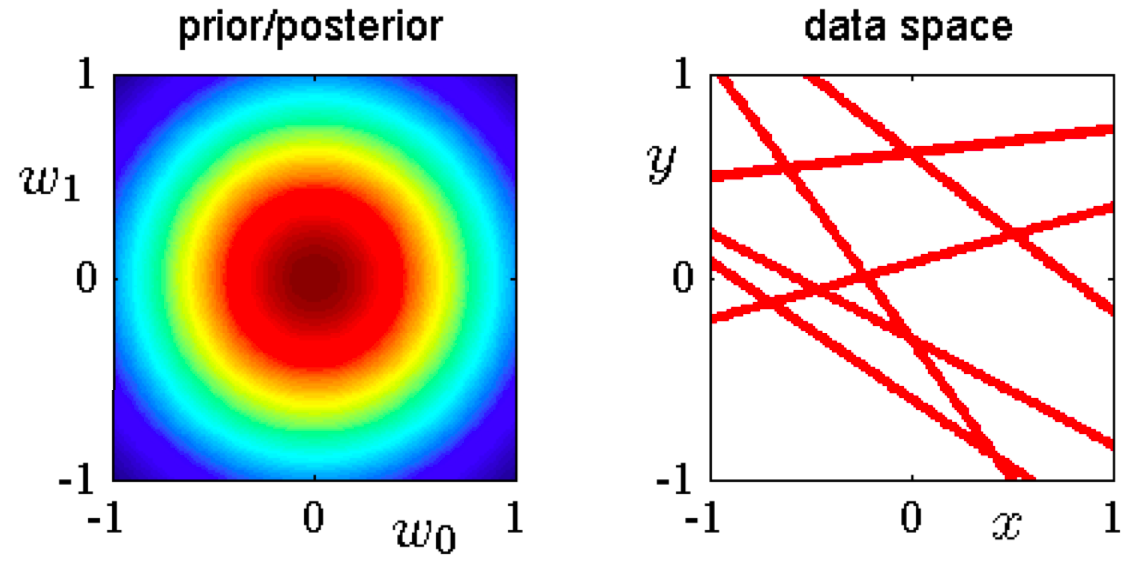
\includegraphics[width=0.6\textwidth]{figs/lin-regression-prior-PRMLFig3-7}
\par\end{center}

\pause{}
\begin{itemize}
\item On right,  $y(x)=\ex\left[y\mid x,w\right]=w_{0}+w_{1}x$, for randomly
chosen $w\sim p(w)=\cn\left(0,\frac{1}{2}I\right)$. 
\end{itemize}
\let\thefootnote\relax\footnotetext{\tiny{Bishop's PRML Fig 3.7}}
\end{frame}
%
\begin{frame}{Example in 1-Dimension: 1 Observation}
\begin{center}
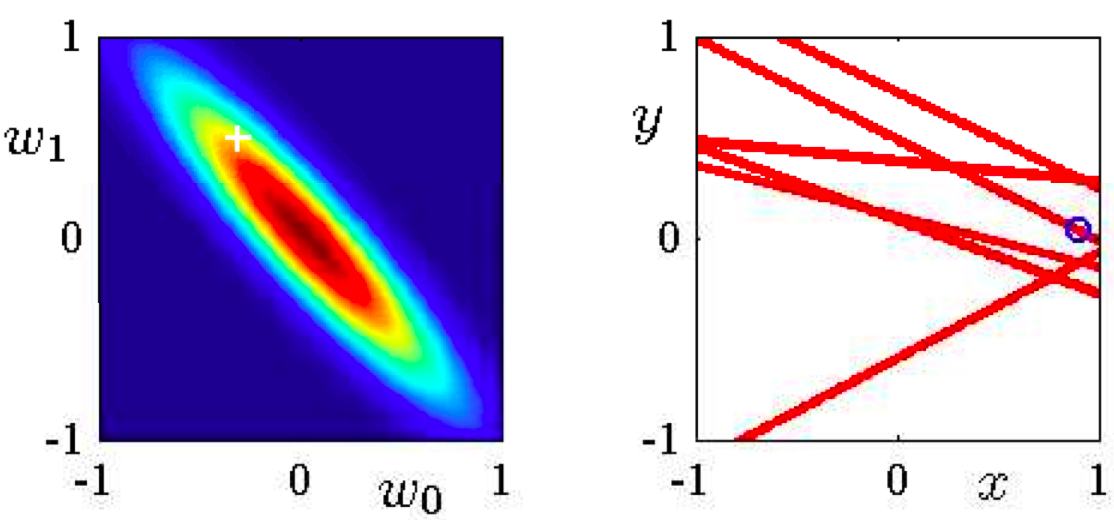
\includegraphics[width=0.6\textwidth]{{figs/lin-regression-prior-PRMLFig3-7.1pt}.png}
\par\end{center}
\begin{itemize}
\item On left: posterior distribution; white '+' indicates true parameters
\item On right: 
\begin{itemize}
  \item blue circle indicates the training observation
  \item red lines,  $y(x)=\ex\left[y\mid x,w\right]=w_{0}+w_{1}x$, for randomly
  chosen $w\sim p(w | \cd )$ (posterior)
\end{itemize}

\end{itemize} 
\let\thefootnote\relax\footnotetext{\tiny{Bishop's PRML Fig 3.7}}
\end{frame}
%
\begin{frame}{Example in 1-Dimension: 2 and 20 Observations}
\begin{center}
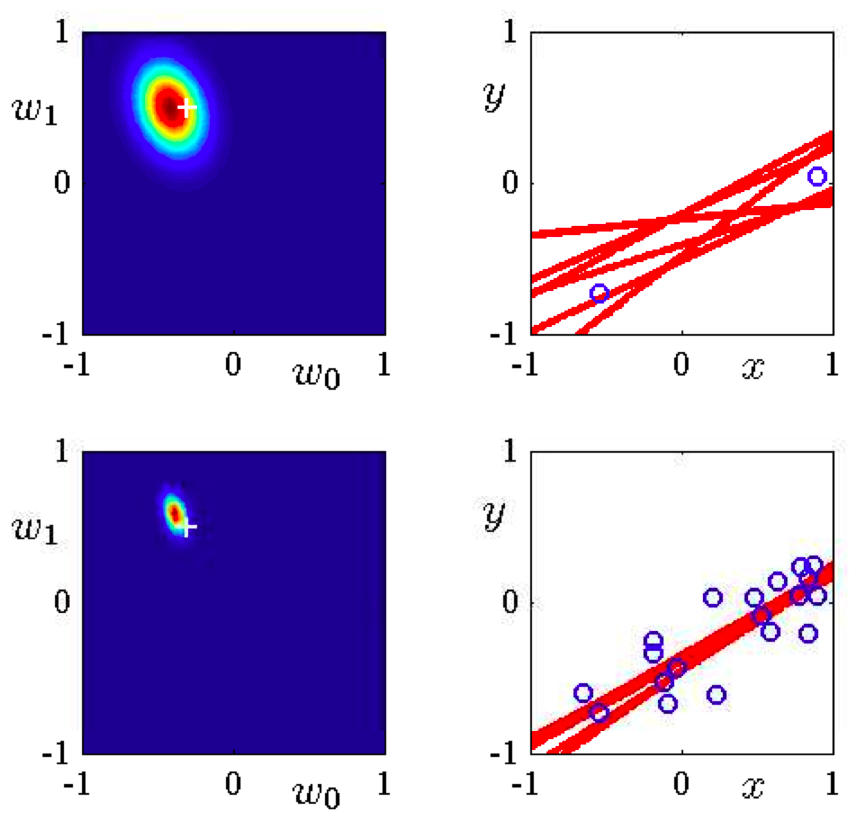
\includegraphics[height=0.7\textheight]{{figs/lin-regression-prior-PRMLFig3-7.2and20pt}.png}
\par\end{center}

\let\thefootnote\relax\footnotetext{\tiny{Bishop's PRML Fig 3.7}}
\end{frame}
%

\section{Gaussian Regression Continued}
\begin{frame}{Closed Form for Posterior}
\begin{itemize}
\item Model:
\begin{eqnarray*}
w & \sim & \cn\left(0,\Sigma_{0}\right)\\
\pause y_{i}\mid x,w & \text{i.i.d.} & \cn(w^{T}x_{i},\sigma^{2})
\end{eqnarray*}


\pause{}
\item Design matrix $X$ $\qquad$Response column vector $y$

\pause{}
\item \textbf{Posterior distribution is a Gaussian distribution:
\begin{eqnarray*}
w\mid\cd & \sim & \pause\cn(\mu_{P},\Sigma_{P})\\
\mu_{\text{P}} & = & \left(X^{T}X+\sigma^{2}\Sigma_{0}^{-1}\right)^{-1}X^{T}y\\
\Sigma_{\text{P}} & = & \left(\sigma^{-2}X^{T}X+\Sigma_{0}^{-1}\right)^{-1}
\end{eqnarray*}
}

\pause{}
\item \textbf{Posterior Variance} $\Sigma_{P}$ gives us a natural \textbf{uncertainty
measure.}
\end{itemize}

\end{frame}
%
\begin{frame}{Closed Form for Posterior}
\begin{itemize}
\item \textbf{Posterior distribution is a Gaussian distribution:
\begin{eqnarray*}
w\mid\cd & \sim & \pause\cn(\mu_{P},\Sigma_{P})\\
\mu_{\text{P}} & = & \left(X^{T}X+\sigma^{2}\Sigma_{0}^{-1}\right)^{-1}X^{T}y\\
\Sigma_{\text{P}} & = & \left(\sigma^{-2}X^{T}X+\Sigma_{0}^{-1}\right)^{-1}
\end{eqnarray*}
}

\pause{}
\item If we want point estimates of $w$\textbf{, MAP estimator} and the
\textbf{posterior mean} are given by
\[
\pause\hat{w}=\mu_{P}=\left(X^{T}X+\sigma^{2}\Sigma_{0}^{-1}\right)^{-1}X^{T}y
\]
 

\pause{}
\item For the prior variance $\Sigma_{0}=\frac{\sigma^{2}}{\lambda}I$,
we get
\[
\hat{w}=\mu_{P}=\left(X^{T}X+\lambda I\right)^{-1}X^{T}y,\pause
\]
which is of course the ridge regression solution. 
\end{itemize}
\end{frame}
%
\begin{frame}{Posterior Mean and Posterior Mode (MAP)}
\begin{itemize}
\item Let's find $\hat{w}_{\text{MAP}}$ another way to elaborate on connection
to ridge.

\pause{}
\item \textbf{Posterior density }on $w$\textbf{ }for\textbf{ }$\Sigma_{0}=\frac{\sigma^{2}}{\lambda}I$:\textbf{
\begin{eqnarray*}
p(w\mid\cd) & \propto & \underbrace{\exp\left(-\frac{\lambda}{2\sigma^{2}}\|w\|^{2}\right)}_{\text{prior}}\underbrace{\prod_{i=1}^{n}\exp\left(-\frac{(y_{i}-w^{T}x_{i})^{2}}{2\sigma^{2}}\right)}_{\text{likelihood}}
\end{eqnarray*}
}

\pause{}
\item To find \textbf{MAP}, sufficient to minimize the negative log posterior:
\begin{eqnarray*}
\hat{w}_{\text{MAP}} & = & \argmin_{w\in\reals^{d}}\left[-\log p(w\mid\cd)\right]\\
\pause & = & \argmin_{w\in\reals^{d}}\underbrace{\sum_{i=1}^{n}(y_{i}-w^{T}x_{i})^{2}}_{\text{log-likelihood}}+\underbrace{\lambda\|w\|^{2}}_{\text{log-prior}}
\end{eqnarray*}


\pause{}
\item Which is the ridge regression objective.
\end{itemize}
\end{frame}
%
\begin{frame}{Predictive Distribution}
\begin{itemize}
\item Given a new input point $x_{\text{new}}$, how to predict $y_{\text{new}}$
?

\pause{}
\item \textbf{Predictive distribution
\begin{eqnarray*}
p(y_{\text{new}}\mid x_{\text{new}},\cd) & = & \pause\int p(y_{\text{new}}\mid x_{\text{new}},w,\cd)p(w\mid\cd)\,dw\\
\pause & = & \int p(y_{\text{new}}\mid x_{\text{new}},w)p(w\mid\cd)\,dw
\end{eqnarray*}
}

\pause{}
\item For Gaussian regression, predictive distribution has closed form.
\end{itemize}
\end{frame}
%
\begin{frame}{Closed Form for Predictive Distribution}
\begin{itemize}
\item \textbf{Model}:
\begin{eqnarray*}
w & \sim & \cn\left(0,\Sigma_{0}\right)\\
\pause y_{i}\mid x,w & \text{i.i.d.} & \cn(w^{T}x_{i},\sigma^{2})
\end{eqnarray*}


\pause{ }
\item \textbf{Predictive Distribution}
\begin{eqnarray*}
p(y_{\text{new}}\mid x_{\text{new}},\cd) & = & \int p(y_{\text{new}\text{ }}\mid x_{\text{new}},w)p(w\mid\cd)\,dw.
\end{eqnarray*}

\begin{itemize}
\item Averages over prediction for each $w$, weighted by posterior distribution.

\pause{ }
\end{itemize}
\item \textbf{Closed form:}
\begin{eqnarray*}
y_{\text{new}}\mid x_{\text{new}},\cd & \sim & \cn\left(\eta_{\text{new}}\,,\,\sigma_{\text{new}}^{2}\right)\\
\pause\eta_{\text{new}} & = & \mu_{\text{P}}^{T}x_{\text{new}}\\
\pause\sigma_{\text{new}}^{2} & = & \underbrace{x_{\text{new}}^{T}\Sigma_{\text{P}}x_{\text{new}}}_{\text{from variance in }w}+\underbrace{\sigma^{2}}_{\text{inherent variance in }y}
\end{eqnarray*}
\end{itemize}
\end{frame}
%
\begin{frame}{Predictive Distributions}
\begin{itemize}
\item With predictive distributions, can give mean prediction with error
bands:
\end{itemize}
\begin{center}
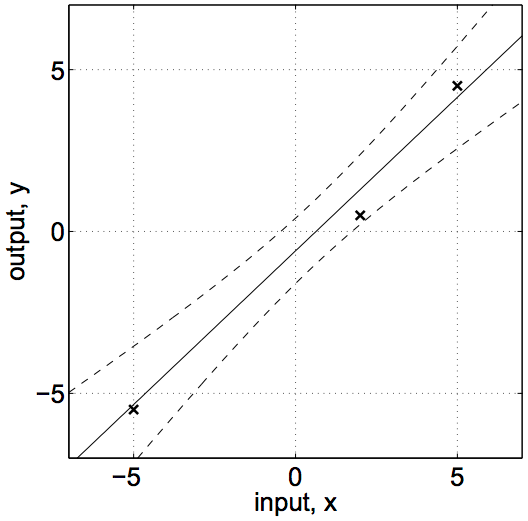
\includegraphics[height=0.7\textheight]{figs/predictiveDistWithErrorBands}
\par\end{center}

\let\thefootnote\relax\footnotetext{\tiny{Rasmussen and Williams' \emph{Gaussian Processes for Machine Learning}, Fig.2.1(b) }}
\end{frame}

\end{document}
